\documentclass[12pt,a4paper,oneside]{report}
\usepackage[utf8]{inputenc}
\usepackage[T1]{fontenc}
\usepackage{amsmath}
\usepackage{amsfonts}
\usepackage{amssymb}
\usepackage{graphicx}
\usepackage{fontspec}
\usepackage{titlesec}
\usepackage{tocloft}
\usepackage[margin=2.5cm]{geometry}
\usepackage{lipsum}
\usepackage[skip=10pt]{parskip}
\usepackage{mwe,tikz}

\ifdefined\EasyMarkPrivateBuild
	\input{private.tex}
	\newcommand{\IfPrivateBuild}[2]{#1}
\else
	\newcommand{\IfPrivateBuild}[2]{#2}
\fi

\setcounter{secnumdepth}{3}
\addtolength{\textwidth}{-1cm}
\addtolength{\oddsidemargin}{1cm}
\addtolength{\evensidemargin}{1cm}

% Calibri or sans-serif as default font
\defaultfontfeatures{Mapping=tex-text,Scale=MatchLowercase}
\IfFontExistsTF{Calibre}{
	\setmainfont{Calibre}
}{
	\renewcommand{\familydefault}{\sfdefault}
}

% TOC horizontal spacing
\cftsetindents{chapter}{0cm}{1cm}
\cftsetindents{section}{1cm}{1cm}
\cftsetindents{subsection}{2cm}{1.2cm}

% TOC vertical spacing
\renewcommand{\cftchapfont}{
	\bfseries
	\fontsize{13pt}{13pt}
	\selectfont
	\vspace{6pt}
}
\cftbeforechapskip12pt
\renewcommand{\cftsecfont}{
	\fontsize{11pt}{11pt}
	\selectfont
	\vspace{6pt}
}
\cftbeforesecskip6pt
\renewcommand{\cftsubsecfont}{
	\fontsize{10pt}{10pt}
	\selectfont
	\vspace{3pt}
}
\cftbeforesubsecskip6pt

% TOC title
\renewcommand\cfttoctitlefont{
	\hfill
	\fontsize{16pt}{16pt}
	\selectfont
	\bfseries
}
\cftbeforetoctitleskip6pt
\cftaftertoctitleskip12pt

% Title format for chapter, section, sub- and subsubsection
% See https://tex.stackexchange.com/questions/511981/titlesec-vertical-align-chapter-and-section
% The -5pt is just pixel pushing bc I couldn't figure out why my chapter/section/subsection/subsubsection headings are slightly indented
\titleformat{\chapter}[hang]{
	\normalfont
	\bfseries
	\filright
	\fontsize{16pt}{16pt}
	\selectfont
}{
	\makebox[1.7cm][l]{\thechapter}
}{0em}{}
\titlespacing{\chapter}{-5pt}{18pt}{12pt}

\titleformat{\section}[hang]{
	\normalfont
	\bfseries
	\filright
	\fontsize{14pt}{14pt}
	\selectfont
}{
	\makebox[1.7cm][l]{\thesection}
}{0em}{}
\titlespacing{\section}{-5pt}{18pt}{12pt}

\titleformat{\subsection}[hang]{
	\normalfont
	\bfseries
	\filright
	\fontsize{12pt}{12pt}
	\selectfont
}{
	\makebox[1.7cm][l]{\thesubsection}
}{0em}{}
\titlespacing{\subsection}{-5pt}{18pt}{12pt}

\titleformat{\subsubsection}[hang]{
	\normalfont
	\bfseries
	\filright
	\fontsize{11pt}{11pt}
	\selectfont
}{
	\makebox[1.7cm][l]{\thesubsubsection}
}{0em}{}
\titlespacing{\subsubsection}{-5pt}{12pt}{12pt}

\newcommand{\IncludeSchoolTemplate}[2]{
	\vspace*{-7em}
	\makebox[\textwidth]{
		\begin{tikzpicture}[
			every node/.style={anchor=north west,inner sep=0pt},
			x=1mm, y=1mm]
			\node (templatepage) at (0,0)
				{\includegraphics[width=\paperwidth,page=#1]{summary.pdf}};
			#2
		\end{tikzpicture}
	}
	\newpage
}


\title{Easy Mark One}
\author{\IfPrivateBuild{\EmRealAuthorName}{T0astBread}}

\begin{document}
	\pagenumbering{gobble}
	\maketitle
	\tableofcontents
	\newpage
	\IfPrivateBuild{
		\IncludeSchoolTemplate{1}{
			\node at (77,-28)
				{Informatik};
			\node at (77,-63)
				{\EmRealAuthorName};
			\node at (77,-80)
				{2019/20};
			\node at (77,-92)
				{Easy Mark One};
			\node at (77,-109)
				{\EmPartner};
			\node at (77,-127) [text width=305,align=justify] {
				\fontsize{12pt}{12pt}
				\selectfont
				\par
				Ziel des Projekts war die Entwicklung eines Tools zur Teilautomatisierung des Bewertungsprozesses für Programmier(haus)aufgaben in der Programmiersprache Java (Teilprojekt \emph{Automark}), sowie einer Web-Plattform für Lehrer und Schüler, um Informationen zu Aufgaben und Bewertungen zu teilen (Teilprojekt \emph{EasyMark}).
				\vskip10pt
				\par
				Alle Programme sollten in Java realisiert werden.
			};
			\node at (77,-174) [text width=300,align=justify] {
				\fontsize{12pt}{12pt}
				\selectfont
				\par
				Automark wurde als ein zusammenhängendes Java-Programm umgesetzt, das über die Kommandozeile sowie über eine GUI gesteuert werden kann. Diverse Libraries wurden für die zahlreichen Funktionen verwendet.
				\vskip10pt
				\par
				EasyMark wurde auf Basis des \emph{Javalin} Web-Frameworks entwickelt. Als Datenbank fungiert eine flache JSON-Datei mit Read/Write Lock. Für kryptographische Funktionen wurde Spring Security (als Standalone-Variante) verwendet.
			};
			\node at (77, -222) [text width=300,align=justify] {
				\fontsize{12pt}{12pt}
				\selectfont
				\par
				Automark: Die Teilaufgaben im Bewertungsprozess wurden zuerst implementiert, danach Nebenfunktionen wie Rollback/mark-resolved. Die GUI wurde entwickelt, um den Einstieg ins Programm zu erleichtern. Ebenfalls noch Zusatzfunktionen wie das automatische Versenden von Ergebnis-Emails und der Konfigurations-Wizard.
				\vskip10pt
				\par
				EasyMark: Zuerst wurden das Datenmodell und das Datenbanksystem entwickelt. Die Funktionalität würde zuerst abstrakt implementiert, dann die Business-Logic. Zuletzt wurde die Sicherheit des Servers überarbeitet und ein Programm zur Konfiguration eines Hosts geschrieben.
			};
		}
		\IncludeSchoolTemplate{2}{
			\node at (77,-28)
				{Informatik};
			\node at (77,-69){
				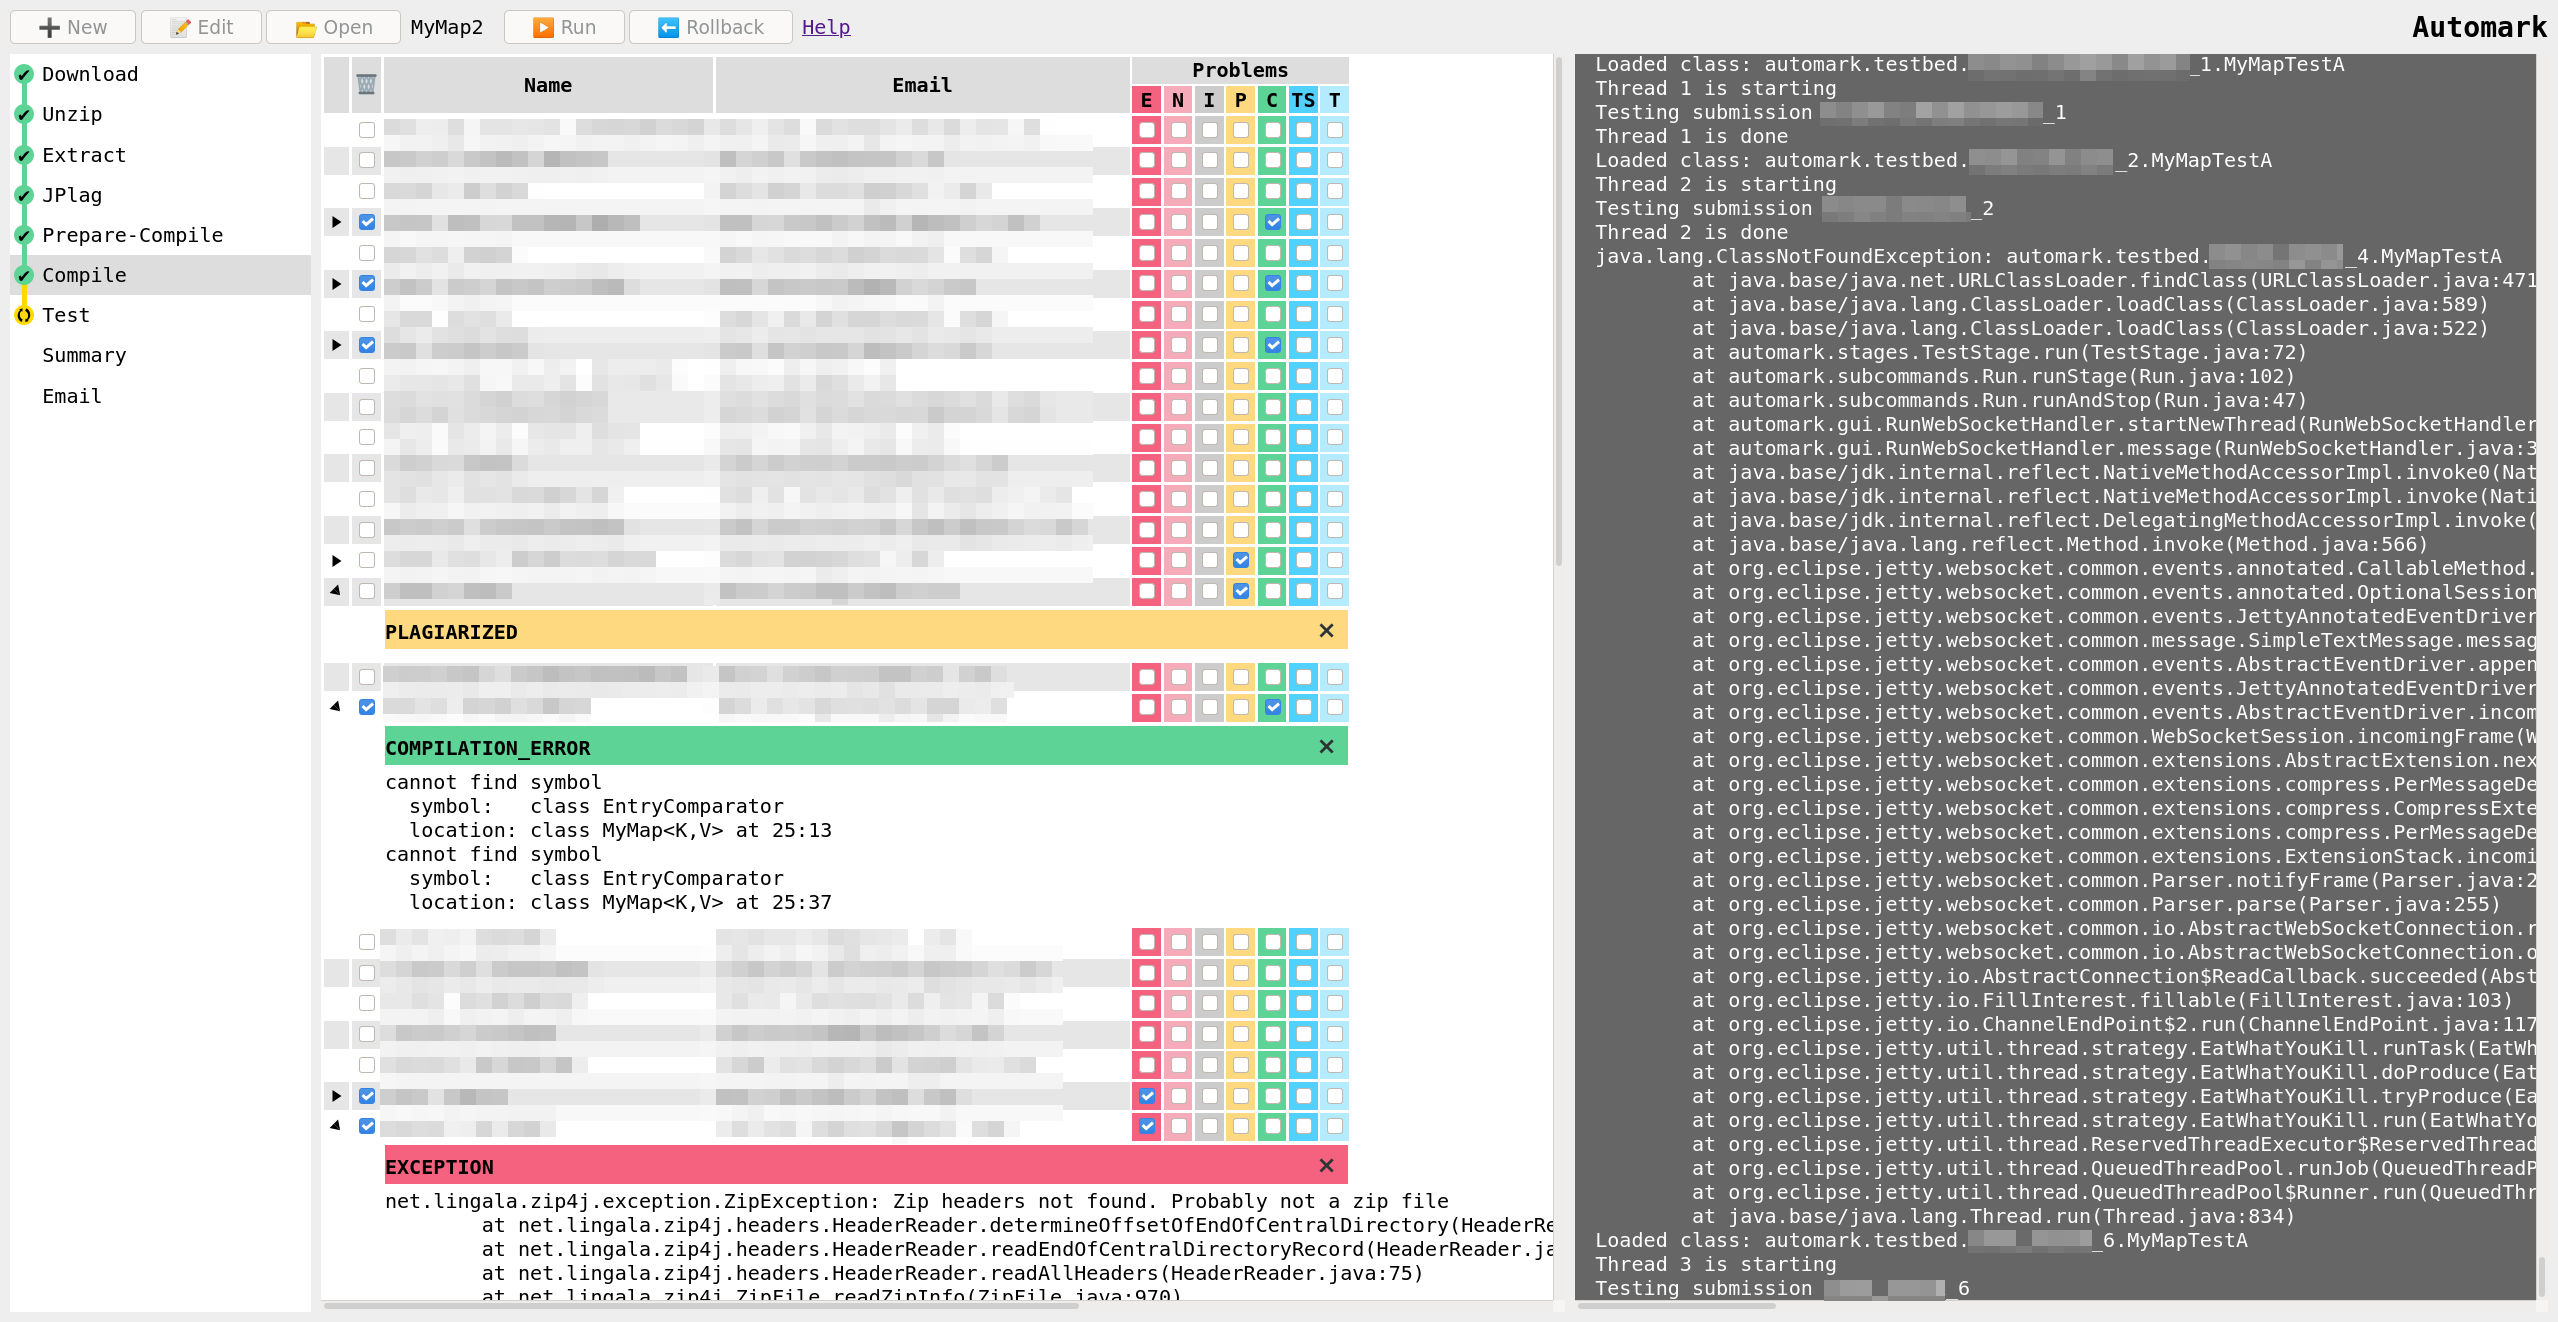
\includegraphics[width=310pt,trim=0pt 0pt 1110pt 0pt,clip]{automark_dashboard_w_details_expanded.png}
			};
			\node at (77,-171) [text width=305,align=center]
				{\emph{Screenshot der Automark-GUI (Ausschnitt). Links befindet sich eine Übersicht über alle Teilaufgaben im Prozess (\emph{Stages}). In der Mitte eine Tablle mit einer Übersicht sowie Details zu Schülerabgaben und deren Mängel. Persönlich identifizierbare Informationen sind unkenntlich gemacht.}};
			\node at (77,-220)
				{--};
			\node at (77,-239)
				{Öffentlich; Bibliothek der \EmSchoolName};
		}
	}{}
	\clearpage
	\pagenumbering{arabic}
	\chapter{Data Chapter 1}
	\section{Data}
	Text text text text text text text text text text text text text text text text text text text text text text text text text.
	As you can see, the header is aligned with the text. I am trying to get the header aligned with the section number while keeping the text aligned with the section title.
	\subsection{Dataset}
	\lipsum
	\subsection{Data Preparation}
	fdfds
	\subsubsection{SQLite}
	fdjksfjdls
	\subsubsection{Data Processing}
	fdjksfjdls
	\subsection{Databases}
	fkdjsfdls
	\subsection{Configuration Data}
	\chapter{More Data}
	\section{Data}
	Yo what's up
\end{document}
